% CREATED BY DAVID FRISK, 2015
\chapter{Methods}
To create the catalog of merge-conflict resolution patterns the following methodology will be used:
\begin{enumerate}
\item Select Merge Commits
\item Classify the merge conflicts
\item Manually identify the corresponding resolution patterns for each classified conflict pattern
\item Autonomously classify each resolution into patterns
\end{enumerate}
\section{Conflict File Tree}
The idea is to find merge-conflict resolution patterns in Git merges. To begin searching for such patterns, we first had to figure out what patterns exist. When looking at the git merge log, using the command git log --merges, it lists the merge commits with the commit messages which could contain a list of conflicting files. However, this approach is not reliable as the commit message could be altered by the commitér who can remove the list of conflicting files. Because of this, we extended the tool to recreate all of the historical merges in the repository to see which conflicts arises. To do this, we first needed to find the two ancestral commits of a merge commit, that is, the two commits that were merged. The following command prints the two commits:
\lstset{language=Bash}
\begin{lstlisting}[frame=single]
git --no-pager log --merges --format=%p <SHA-1> | head -n1
\end{lstlisting}
where <SHA-1> is the merge commit SHA-1. We then parse the two commits and performs the merge using the following sequence of commands. The two commits are hereby referred to as C1 and C2:\\
\lstset{language=Bash}
\begin{lstlisting}[frame=single]
git reset --hard <SHA-1 of C1>
git clean -f
git branch <temp branch name>
git checkout <SHA-1 of C2>
git merge <temp branch name>
\end{lstlisting}
In 1, we set HEAD to commit C1 and changes the working copy to the state of that commit. In 2,  the working copy is cleaned to be ready for the merge. In 3, a new branch is created which points at commit C1. In 4, we checkout commit C2. In 5, we merge the two commits by merging the newly created branch into commit C2. Git will now print out the conflicting files, which we then can parse. Afterwards, we abort the merge and delete the branch.
\paragraph*{}
The common ancestor-, local- and remote file, along with the resulting resolution file in the merge commit, are copied and saved in the Conflict file tree. The Conflict File Tree consist of folders and the versions of the conflicting files, structured according to the figure below.\\
\begin{figure}[H]
\centering
%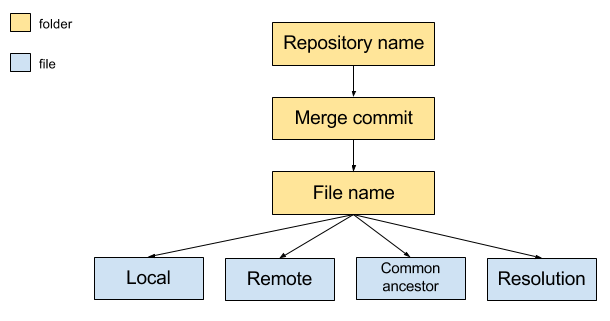
\includegraphics[width=0.45\linewidth, trim=3cm 11cm 3cm 11cm]{figure/conflicts.png}
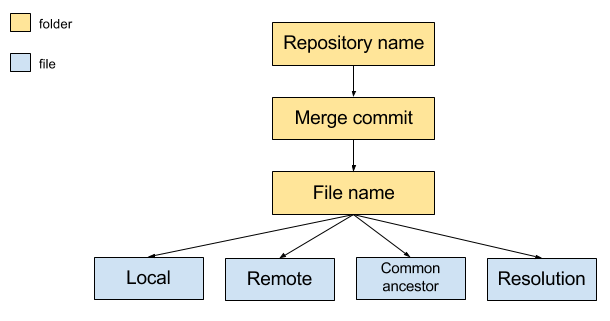
\includegraphics[width=400pt]{figure/conflicts.png}
\caption{Showing the structure of a Conflict File Tree}
\end{figure}

Having all the conflicting file versions in a structured manner will make it easier to analyse them further.

\section{Selection of Merge Commits}
To get a good sample of merge commits, we will clone each project and list all historical merges using the command “git --no-pager log --merges”. This command lists all merge commits in a project and allows for specification of exactly what information we are interested in. This includes the commit SHA-1, parent commits, commit message etc. For each merge commit, we will reproduce the merge using SSMerge and use all conflicts that it encounters. That is, the conflicts that even a semantical and syntactical merge tool is unable to solve automatically.
\section{Classify Merge Conflicts}
To classify conflicts, we aim to use the tool Conflicts Analyzer developed by Accioly(source). This tool automatically clones Github projects and performs the historical merges of the projects using the merge tool SSMerge(source), which is a semistructured merge tool. When semantic merge-conflicts occur, Conflicts Analyzer classifies them according to the conflict patterns defined by Accioly which is listed in table (no) in the pre study chapter.
\section{Identify Resolution Patterns}
For each conflict pattern, we will strive to identify the different corresponding resolution patterns. We will try to identify patterns that cover all ways of resolving each type of conflict. For example, the ModifierList conflict pattern requires the resolution to choose which modifiers to use. Let's assume a case where the common ancestor has the modifier “protected”, one revision has changed it to “private” and one has changed it to “public”. One pattern here may be to always choose the least restrictive one, namely the “public”, to reduce the chance of introducing an error. On the other hand, one pattern could be that the “private” modifier is chosen to increase information hiding, which is often desired in object oriented programming.
\paragraph*{}
A conflict pattern can have one or many resolution patterns. Likewise, a resolution pattern might solve one or more conflict patterns. We will create a catalog of these resolution patterns and map them to their corresponding conflict patterns. Below is an example of how the catalog could be formated:\\
\begin{tabular}{ p{8cm} p{6cm} }
\hline
\multicolumn{1}{c}{\textbf{Pattern}} & \multicolumn{1}{c}{\textbf{Description}}\\
ModifiedList &
\begin{itemize}
\item Resolution Pattern \#1
\item Resolution Pattern \#2
\item Resolution Pattern \#3
\end{itemize}
\end{tabular}
\section{Automatic Classification of Each Resolution}
Using the catalog of identified merge-conflict resolution patterns, we will create an infrastructure which autonomously classifies all selected merge conflicts. The infrastructure will mine GitHub projects, starting with the top 20 starred projects listed in table (no). Using the data acquired we will conduct a statistical analysis of the frequency of the resolution patterns.